\documentclass[11pt]{elegantpaper}

\title{Bubble detection}
\author{Chen Jiale}
%\institute{\href{https://github.com/ElegantLaTeX}{Elegant\LaTeX{} Program}}

\version{0.1}
\date{\today}

% cmd for this doc
\usepackage{array}
\newcommand{\ccr}[1]{\makecell{{\color{#1}\rule{1cm}{1cm}}}}

\begin{document}

\maketitle

\begin{abstract}

\keywords{Distributed sensing,network pruning}
\end{abstract}

\setlength{\parindent}{2em}
\section{Comparison of bubble detectors and size distribution estimators}
\subsection*{General}    
Bubble(circular objects) dtection algorithms can be divided into two approaches, geometry-based and appearance-based.

Geometry-based approaches detects parameterized circular objects in the image edge map.

Drawbacks: Sensitive to noise, high false positive rate. 

Appearance-based appraches using sliding window combining with a classier like boosting based, 
Hog based and CNN classifier

Drawbacks: need large amount of training data.

\subsection*{Estimation of bubble size}

\section{results of conventional techniques}
The results of conventional image processin method are as follow:
\begin{figure}[htbp]
	\centering
    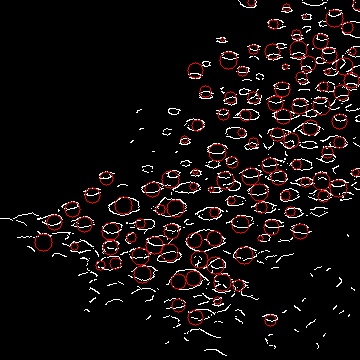
\includegraphics[width=0.2\textwidth]{../results_edge.jpg}
    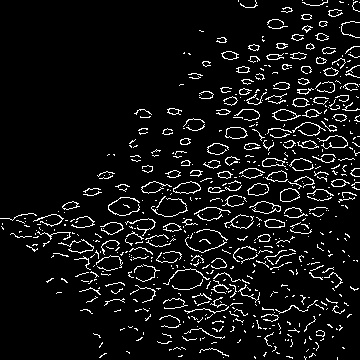
\includegraphics[width=0.2\textwidth]{../edge_0.jpg}
    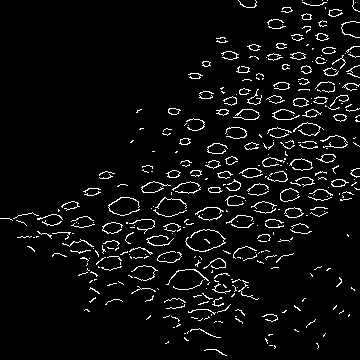
\includegraphics[width=0.2\textwidth]{../edge_1.jpg}
    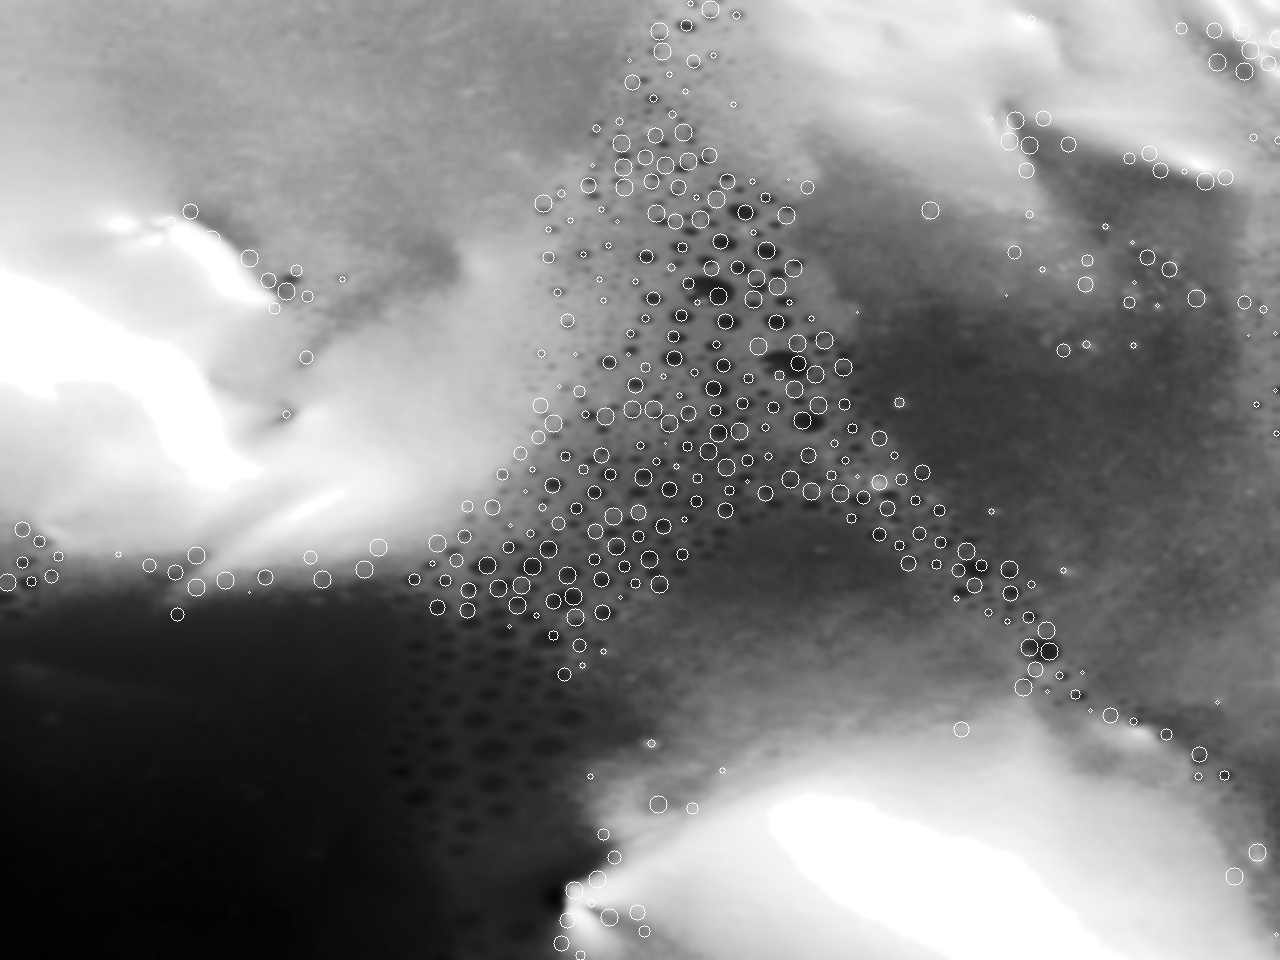
\includegraphics[width=0.4\textwidth]{../results_all.jpg}
\end{figure}

As we can see from the results, bubbles with round extracted edge can be detected. However, the false 
positive rate and false negative rate are relatively high. The problems of hough circle detection can be listed as follows:
\begin{enumerate}
	\item High false positive rate because hough circle detection tends to detect the arcs that can fits in a circular model.
	\item Due to the different angle of view, the extracted edges of some bubble look more like ecllipse rather than a perfect circle.
	The circular bounding box can not perfectly mark out a bubble
	\item The reflection of the surface will cause much false positive detection.
\end{enumerate}

\section{related work}
Jarmo Ilonen and etc has compared the performance of different bubble detection methods,which includes 
circular Hough transform (CHT) method, Concentric Circular Arrangements(CCA),boosting based method and 
CNN method.And the results shows that CNN method outerperform than other methods

They established a dataset, which contains 120 images(72 for training, 48 for testing, 20 images for each rotor speed).Each image is 1482 * 1482 pixel.During training,
they extract each bubble using a 28 * 28 image patch and label it as positive examples. They also implement data augumentation like 
shifting and scaling. In this way,the training data contained 148,860 positive and 317,732 negative examples.

During bubble detection, they use sliding window of different scales as the input of CNN model to detect whether there is a bubble in the window. For lowest scale, the window size is 28 * 28. 
Since only square bounding boxes can be obtained in this way. The author integating the results of each window to form a detection image(detection probability map) 
under a certain scale. After that, they implement connected component analysis on the detection image. They first threshold the detection image into binary image. 
They reject the areas that do not meet the following requirments:
\begin{enumerate}
	\item area is larger than ta
	\item the proportion of the pixels in the convex hull that are one is larger than ts
	\item the ratio of minor and major axis is larger than tm
\end{enumerate}
\begin{figure}[tbp]
    \centering
    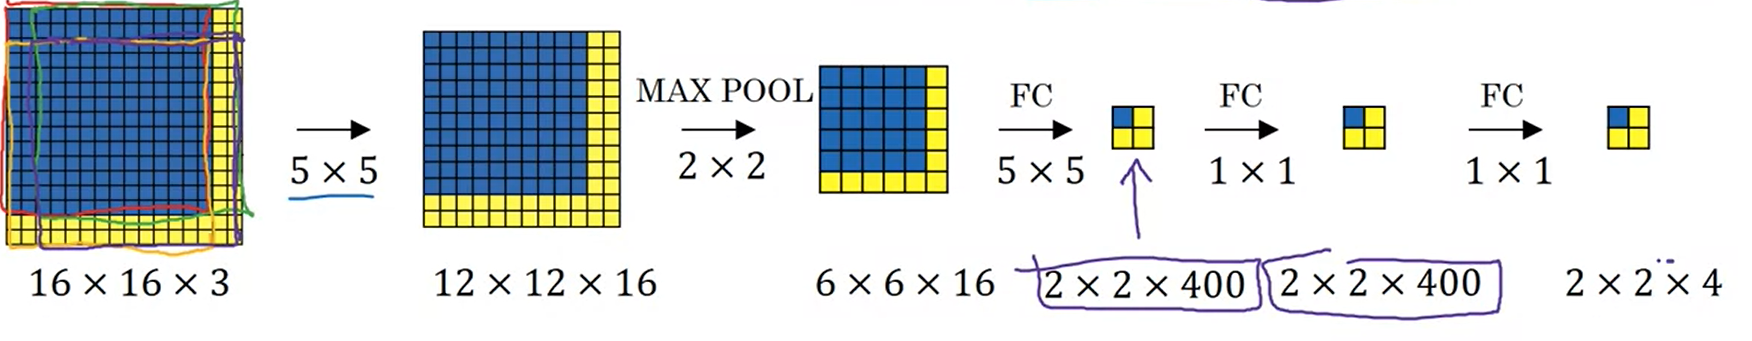
\includegraphics[width=0.8\textwidth]{image/sliding_window.png}
    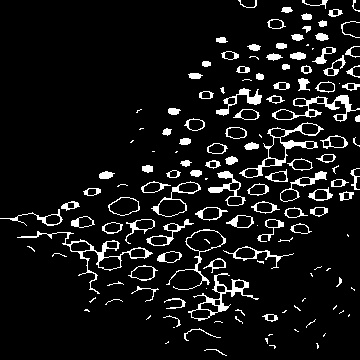
\includegraphics[width=0.4\textwidth]{../close.jpg}
\end{figure}


\section{YOLO}
YOLO is a one stage object detection algorithm. The basic idea of yolo algorithm is also sliding windows. First, the image is split into multiple grids. As shown in the image, 13 by 13 grid is used.
The final output of yolo is a  13 * 13 *(B*(5+C)) tensor. It means each grid corresponds to a pixel in final 13 * 13 feature map. The dimension of each pixel is (B*(5+C)). If we assume only one bounding box is detected in one grid 
and we only want to detect 3 classes, the final ouput can be written as $[P, bx,by,bw,bh,c1,c2,c3]$. During training phase, only the grid that the center of the GT box falls into are resbosible for detecting the object. In other words,
the grid which contains the centroids of the GT bounding box is labeled as $[1, bx,by,bw,bh,c1,c2,c3]$

\begin{figure}[htbp]
	\centering
    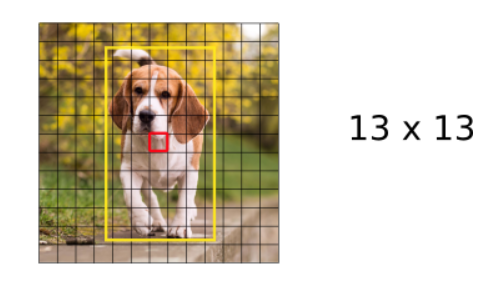
\includegraphics[width=0.6\textwidth]{image/dog.png}
    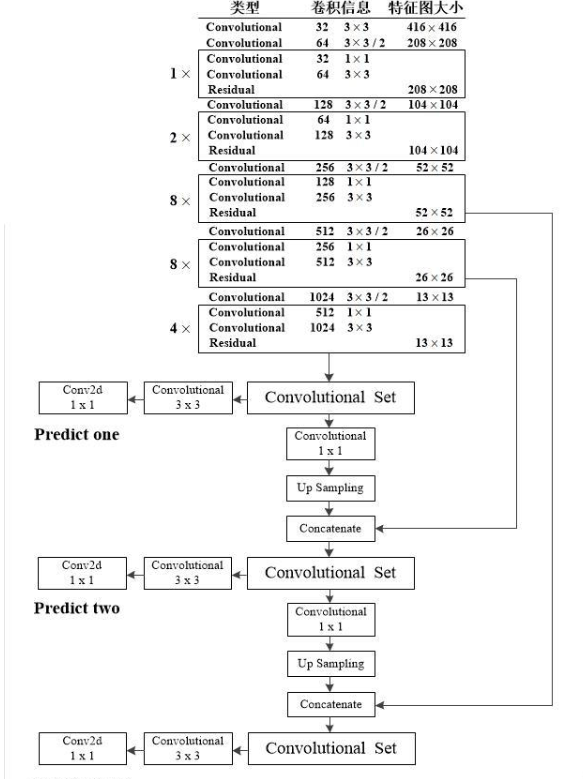
\includegraphics[width=0.6\textwidth]{image/yolo.png}

\end{figure}


\section{faster rcnn}
The basic idea of faster rcnn is to using the RPN(region proposal network) to find the region of interest and use the region of interest as the input of 
CNN network to obtain the classification results. The basic structure of faster rcnn are shown in the follow figure. First, input the image to a convolutional layer 
to extract the features of the image. The features are used to obtained the bounding box proposal in the original image. Using the bounding box proposal and the features
we can select the feature map inside the bounding box proposal and input them into the fully connected layer the detect which object is. 
\begin{figure}[htbp]
    \centering
    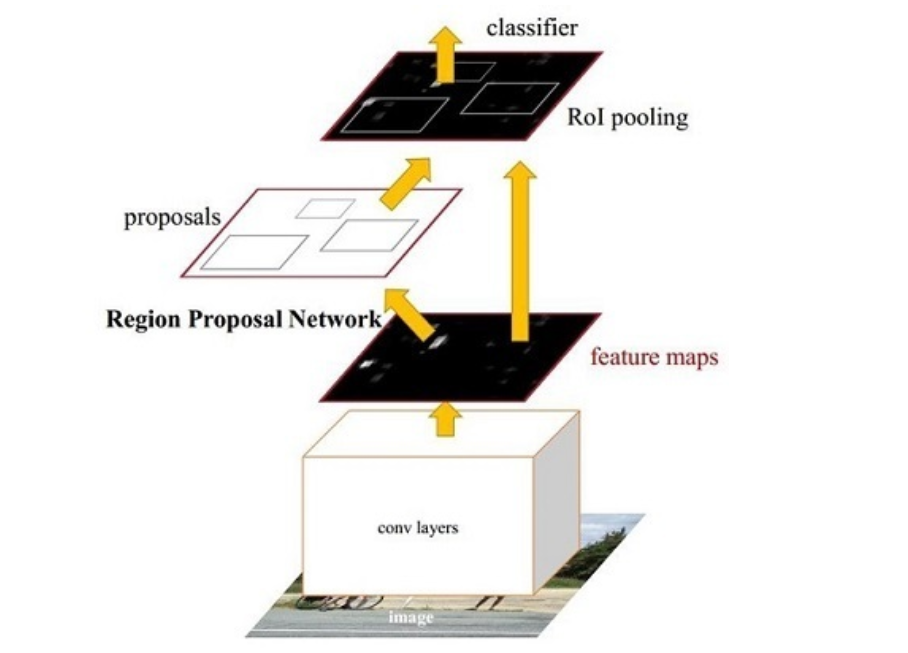
\includegraphics[width=0.6\textwidth]{image/fasterrcnn.png}
    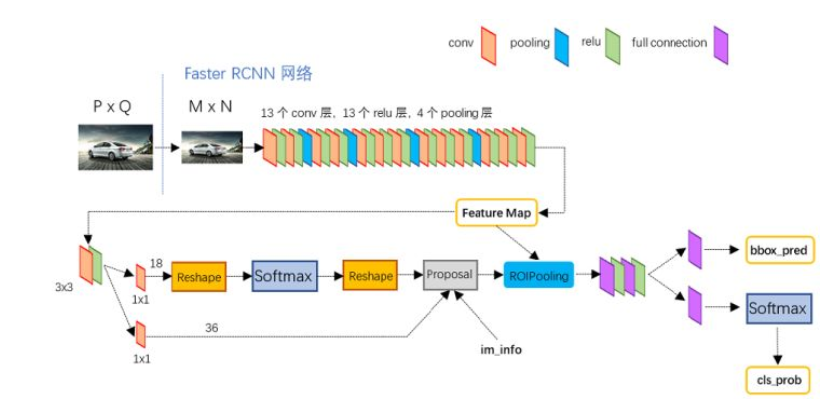
\includegraphics[width=0.6\textwidth]{image/faster_rcnn_1.png}
\end{figure}

\section{System}
Considering that we cannot obtain enough data and labelling the exact shape of each bubble is diffcult. I tend to construct the algorithm as follows:

\begin{enumerate}
	\item Using sliding windows to generate small images and manually label them as bubble or no bubble.
	\item Build a convolutional model that can output detection map of different scales using the data above 
	\item Extracts the bounding box of bubble based on the detection image.
\end{enumerate}

    
\end{document}